\documentclass{standalone}
\usepackage{tikz}
\usetikzlibrary{patterns, positioning}
\usepackage[sfdefault]{ClearSans} %% option 'sfdefault' activates Clear Sans as the default text font
\usepackage[T1]{fontenc}

\begin{document}
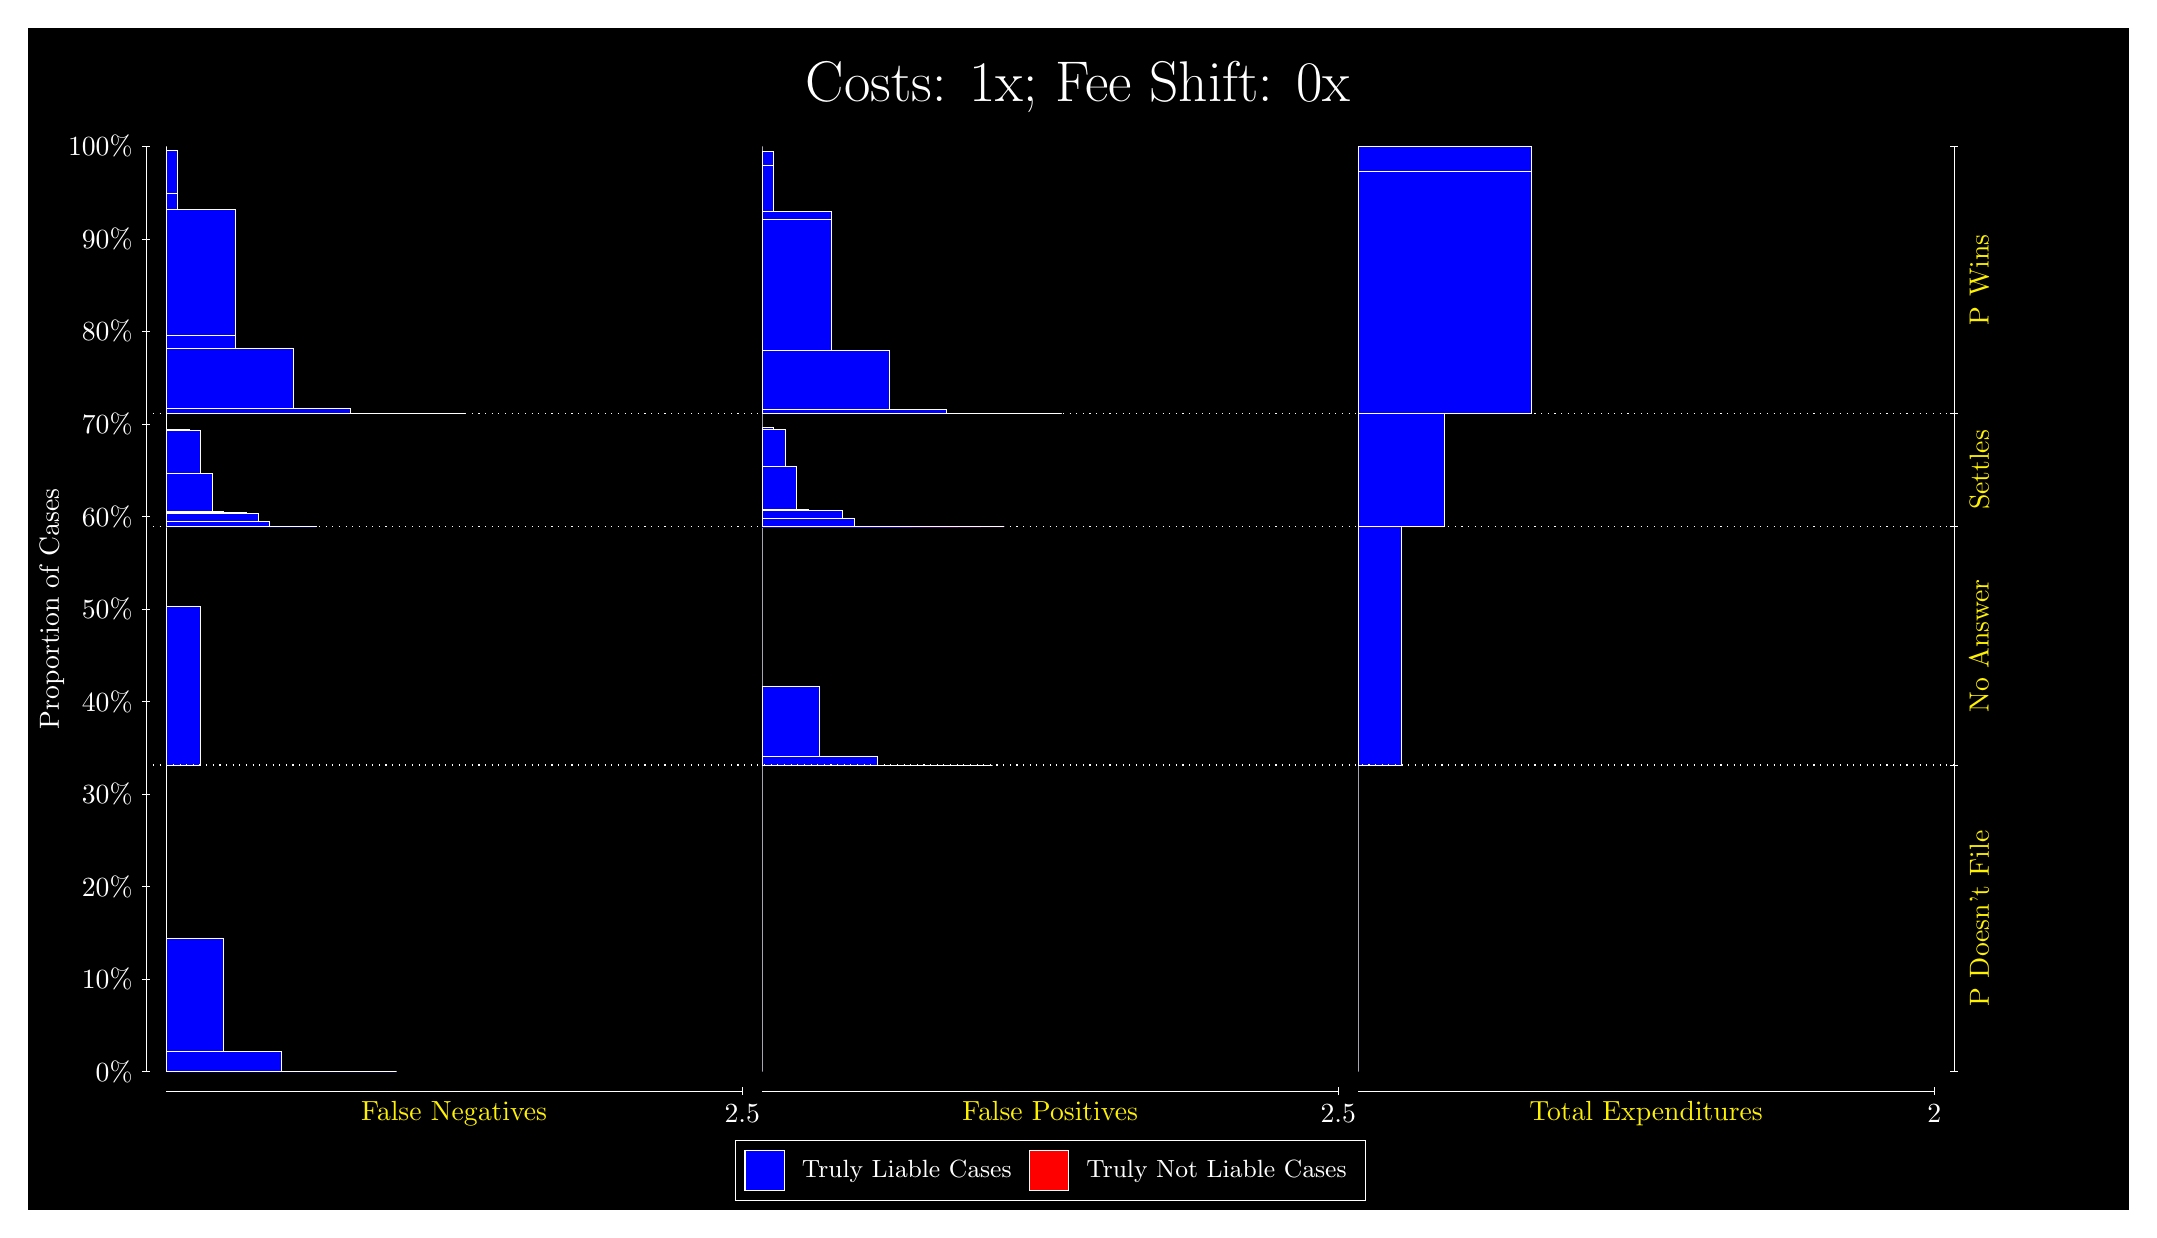
\begin{tikzpicture}
\draw[fill=black] (0,0) rectangle (26.667,15);
\draw[text=white] (0,13.5) rectangle (26.667,15) node[midway] {\huge Costs: 1x; Fee Shift: 0x};
\draw[white, very thin] (1.5,1.75) -- (1.5,13.5);
\node[rotate=90, text=white, anchor=center] at (0.3, 7.625) {Proportion of Cases};
\draw[white, very thin] (1.45,1.75) -- (1.55,1.75);
\node[text=white, anchor=east] at (1.45, 1.75) {0\%};
\draw[white, very thin] (1.45,2.925) -- (1.55,2.925);
\node[text=white, anchor=east] at (1.45, 2.925) {10\%};
\draw[white, very thin] (1.45,4.1) -- (1.55,4.1);
\node[text=white, anchor=east] at (1.45, 4.1) {20\%};
\draw[white, very thin] (1.45,5.275) -- (1.55,5.275);
\node[text=white, anchor=east] at (1.45, 5.275) {30\%};
\draw[white, very thin] (1.45,6.45) -- (1.55,6.45);
\node[text=white, anchor=east] at (1.45, 6.45) {40\%};
\draw[white, very thin] (1.45,7.625) -- (1.55,7.625);
\node[text=white, anchor=east] at (1.45, 7.625) {50\%};
\draw[white, very thin] (1.45,8.8) -- (1.55,8.8);
\node[text=white, anchor=east] at (1.45, 8.8) {60\%};
\draw[white, very thin] (1.45,9.975) -- (1.55,9.975);
\node[text=white, anchor=east] at (1.45, 9.975) {70\%};
\draw[white, very thin] (1.45,11.15) -- (1.55,11.15);
\node[text=white, anchor=east] at (1.45, 11.15) {80\%};
\draw[white, very thin] (1.45,12.325) -- (1.55,12.325);
\node[text=white, anchor=east] at (1.45, 12.325) {90\%};
\draw[white, very thin] (1.45,13.5) -- (1.55,13.5);
\node[text=white, anchor=east] at (1.45, 13.5) {100\%};

\draw[white, very thin] (24.457,1.75) -- (24.457,13.5);
\draw[white, very thin] (24.407,1.75) -- (24.507,1.75);
\node[anchor=west] at (24.407, 1.75) {};
\draw[white, very thin] (24.407,5.6427) -- (24.507,5.6427);
\node[anchor=west] at (24.407, 5.6427) {};
\draw[white, very thin] (24.407,8.6702) -- (24.507,8.6702);
\node[anchor=west] at (24.407, 8.6702) {};
\draw[white, very thin] (24.407,10.111) -- (24.507,10.111);
\node[anchor=west] at (24.407, 10.111) {};
\draw[white, very thin] (24.407,13.5) -- (24.507,13.5);
\node[anchor=west] at (24.407, 13.5) {};

\draw[white, very thin, fill=blue] (1.75,1.75) rectangle (4.6775,1.75);
\draw[white, very thin, fill=blue] (1.75,1.75) rectangle (3.9457,1.7521);
\draw[white, very thin, fill=blue] (1.75,1.7521) rectangle (3.2138,2.0018);
\draw[white, very thin, fill=blue] (1.75,2.0018) rectangle (2.4819,3.4429);
\draw[white, very thin, fill=red] (1.75,3.4429) rectangle (1.75,3.4429);
\draw[white, very thin, fill=blue] (1.75,3.4429) rectangle (1.75,5.6427);
\draw[white, very thin, fill=blue] (1.75,5.6427) rectangle (2.1891,7.6649);
\draw[white, very thin, fill=red] (1.75,7.6649) rectangle (1.75,7.6649);
\draw[white, very thin, fill=blue] (1.75,7.6649) rectangle (1.75,8.6702);
\draw[white, very thin, fill=blue] (1.75,8.6702) rectangle (3.6529,8.6704);
\draw[white, very thin, fill=blue] (1.75,8.6704) rectangle (3.0674,8.7325);
\draw[white, very thin, fill=blue] (1.75,8.7325) rectangle (2.921,8.8372);
\draw[white, very thin, fill=blue] (1.75,8.8372) rectangle (2.7746,8.8503);
\draw[white, very thin, fill=blue] (1.75,8.8503) rectangle (2.4819,8.8682);
\draw[white, very thin, fill=blue] (1.75,8.8682) rectangle (2.3355,9.3431);
\draw[white, very thin, fill=blue] (1.75,9.3431) rectangle (2.1891,9.8958);
\draw[white, very thin, fill=blue] (1.75,9.8958) rectangle (2.0428,9.9012);
\draw[white, very thin, fill=red] (1.75,9.9012) rectangle (1.75,9.9012);
\draw[white, very thin, fill=blue] (1.75,9.9012) rectangle (1.75,10.111);
\draw[white, very thin, fill=blue] (1.75,10.111) rectangle (5.5558,10.111);
\draw[white, very thin, fill=blue] (1.75,10.111) rectangle (4.8239,10.111);
\draw[white, very thin, fill=blue] (1.75,10.111) rectangle (4.092,10.168);
\draw[white, very thin, fill=blue] (1.75,10.168) rectangle (3.3602,10.939);
\draw[white, very thin, fill=blue] (1.75,10.939) rectangle (2.6283,11.094);
\draw[white, very thin, fill=blue] (1.75,11.094) rectangle (2.6283,12.701);
\draw[white, very thin, fill=blue] (1.75,12.701) rectangle (1.8964,12.904);
\draw[white, very thin, fill=blue] (1.75,12.904) rectangle (1.8964,13.447);
\draw[white, very thin, fill=red] (1.75,13.447) rectangle (1.75,13.447);
\draw[white, very thin, fill=blue] (1.75,13.447) rectangle (1.75,13.5);
\draw[white, very thin, fill=red] (9.3189,1.75) rectangle (9.3189,1.75);
\draw[white, very thin, fill=blue] (9.3189,1.75) rectangle (9.3189,5.6427);
\draw[white, very thin, fill=red] (9.3189,5.6427) rectangle (12.246,5.6427);
\draw[white, very thin, fill=blue] (9.3189,5.6427) rectangle (12.246,5.6427);
\draw[white, very thin, fill=blue] (9.3189,5.6427) rectangle (11.515,5.6429);
\draw[white, very thin, fill=blue] (9.3189,5.6429) rectangle (10.783,5.7493);
\draw[white, very thin, fill=blue] (9.3189,5.7493) rectangle (10.051,6.6479);
\draw[white, very thin, fill=blue] (9.3189,6.6479) rectangle (9.3189,8.6702);
\draw[white, very thin, fill=red] (9.3189,8.6702) rectangle (12.393,8.6702);
\draw[white, very thin, fill=blue] (9.3189,8.6702) rectangle (12.393,8.6702);
\draw[white, very thin, fill=red] (9.3189,8.6702) rectangle (12.1,8.6702);
\draw[white, very thin, fill=blue] (9.3189,8.6702) rectangle (12.1,8.6702);
\draw[white, very thin, fill=red] (9.3189,8.6702) rectangle (11.807,8.6702);
\draw[white, very thin, fill=blue] (9.3189,8.6702) rectangle (11.807,8.6702);
\draw[white, very thin, fill=blue] (9.3189,8.6702) rectangle (11.661,8.6702);
\draw[white, very thin, fill=blue] (9.3189,8.6702) rectangle (11.368,8.6702);
\draw[white, very thin, fill=red] (9.3189,8.6702) rectangle (11.222,8.6702);
\draw[white, very thin, fill=blue] (9.3189,8.6702) rectangle (11.222,8.6704);
\draw[white, very thin, fill=blue] (9.3189,8.6704) rectangle (11.075,8.6706);
\draw[white, very thin, fill=blue] (9.3189,8.6706) rectangle (10.929,8.6706);
\draw[white, very thin, fill=blue] (9.3189,8.6706) rectangle (10.636,8.6706);
\draw[white, very thin, fill=blue] (9.3189,8.6706) rectangle (10.49,8.7753);
\draw[white, very thin, fill=blue] (9.3189,8.7753) rectangle (10.344,8.8788);
\draw[white, very thin, fill=blue] (9.3189,8.8788) rectangle (10.197,8.8795);
\draw[white, very thin, fill=blue] (9.3189,8.8795) rectangle (9.9044,8.8849);
\draw[white, very thin, fill=blue] (9.3189,8.8849) rectangle (9.758,9.4376);
\draw[white, very thin, fill=blue] (9.3189,9.4376) rectangle (9.6116,9.9125);
\draw[white, very thin, fill=blue] (9.3189,9.9125) rectangle (9.4652,9.9304);
\draw[white, very thin, fill=blue] (9.3189,9.9304) rectangle (9.3189,10.111);
\draw[white, very thin, fill=red] (9.3189,10.111) rectangle (13.125,10.111);
\draw[white, very thin, fill=blue] (9.3189,10.111) rectangle (13.125,10.111);
\draw[white, very thin, fill=red] (9.3189,10.111) rectangle (12.393,10.111);
\draw[white, very thin, fill=blue] (9.3189,10.111) rectangle (12.393,10.111);
\draw[white, very thin, fill=red] (9.3189,10.111) rectangle (11.661,10.111);
\draw[white, very thin, fill=blue] (9.3189,10.111) rectangle (11.661,10.164);
\draw[white, very thin, fill=red] (9.3189,10.164) rectangle (10.929,10.164);
\draw[white, very thin, fill=blue] (9.3189,10.164) rectangle (10.929,10.909);
\draw[white, very thin, fill=blue] (9.3189,10.909) rectangle (10.197,12.572);
\draw[white, very thin, fill=red] (9.3189,12.572) rectangle (10.197,12.572);
\draw[white, very thin, fill=blue] (9.3189,12.572) rectangle (10.197,12.671);
\draw[white, very thin, fill=blue] (9.3189,12.671) rectangle (9.4652,13.254);
\draw[white, very thin, fill=blue] (9.3189,13.254) rectangle (9.4652,13.443);
\draw[white, very thin, fill=blue] (9.3189,13.443) rectangle (9.3189,13.5);
\draw[white, very thin, fill=red] (16.888,1.75) rectangle (16.888,1.75);
\draw[white, very thin, fill=blue] (16.888,1.75) rectangle (16.888,5.6427);
\draw[white, very thin, fill=red] (16.888,5.6427) rectangle (17.437,5.6427);
\draw[white, very thin, fill=blue] (16.888,5.6427) rectangle (17.437,8.6702);
\draw[white, very thin, fill=red] (16.888,8.6702) rectangle (17.986,8.6702);
\draw[white, very thin, fill=blue] (16.888,8.6702) rectangle (17.986,10.111);
\draw[white, very thin, fill=red] (16.888,10.111) rectangle (19.083,10.111);
\draw[white, very thin, fill=blue] (16.888,10.111) rectangle (19.083,13.181);
\draw[white, very thin, fill=red] (16.888,13.181) rectangle (19.083,13.181);
\draw[white, very thin, fill=blue] (16.888,13.181) rectangle (19.083,13.5);
\draw[white, dotted] (1.5,5.6427) -- (24.457,5.6427);
\draw[white, dotted] (1.5,8.6702) -- (24.457,8.6702);
\draw[white, dotted] (1.5,10.111) -- (24.457,10.111);
\draw[white, very thin] (1.75,1.5) -- (9.0689,1.5);
\node[text=yellow, anchor=north] at (5.4094, 1.5) {False Negatives};
\draw[white, very thin] (9.0689,1.45) -- (9.0689,1.55);
\node[text=white, anchor=north] at (9.0689, 1.45) {2.5};

\draw[white, very thin] (9.3189,1.5) -- (16.638,1.5);
\node[text=yellow, anchor=north] at (12.978, 1.5) {False Positives};
\draw[white, very thin] (16.638,1.45) -- (16.638,1.55);
\node[text=white, anchor=north] at (16.638, 1.45) {2.5};

\draw[white, very thin] (16.888,1.5) -- (24.207,1.5);
\node[text=yellow, anchor=north] at (20.547, 1.5) {Total Expenditures};
\draw[white, very thin] (24.207,1.45) -- (24.207,1.55);
\node[text=white, anchor=north] at (24.207, 1.45) {2};

\node[text=yellow, centered, rotate=90] at (24.777, 3.6963) {P Doesn't File};
\node[text=yellow, centered, rotate=90] at (24.777, 7.1564) {No Answer};
\node[text=yellow, centered, rotate=90] at (24.777, 9.3903) {Settles};
\node[text=yellow, centered, rotate=90] at (24.777, 11.805) {P Wins};

\draw (12.978300999999998,1.5) node[draw=none] (baseCoordinate) {};
\begin{scope}[align=center]
        \matrix[scale=0.5, draw=white, below=0.5cm of baseCoordinate, nodes={draw}, column sep=0.1cm]{
            \node[rectangle, draw, minimum width=0.5cm, minimum height=0.5cm, fill=blue] {}; &
            \node[draw=none, font=\small, text=white] (B) {Truly Liable Cases}; &
            \node[rectangle, draw, minimum width=0.5cm, minimum height=0.5cm, fill=red] {}; &
            \node[draw=none, font=\small, text=white] (B) {Truly Not Liable Cases}; \\
            };
\end{scope}

\end{tikzpicture}
\end{document}